\documentclass[11pt]{article}
\usepackage[utf8]{inputenc}  % gebruik de juiste 'character encoding'
\usepackage[english]{babel}    % definitie van de taal (Engels is de standaard)
\usepackage{hyperref}        % geef URLs netjes weer
\usepackage{graphicx} 		 % Invoegen van plaatjes , ref: https://nl.sharelatex.com/learn/Inserting_Images
\usepackage{float} 			% MIJN VERSLAG
\usepackage{pdfpages}

\graphicspath{{image/}}

\title{\huge \textbf{GROW model, coaching session 1}}
\date{$9^{th}$ of May 2019}

\setlength\parindent{0pt} 	% geen irritant indents bij de paragraph

\begin{document}
	
	\thispagestyle{empty}
	
	\maketitle
	
	
	\begin{figure}[!h]
		\centering
		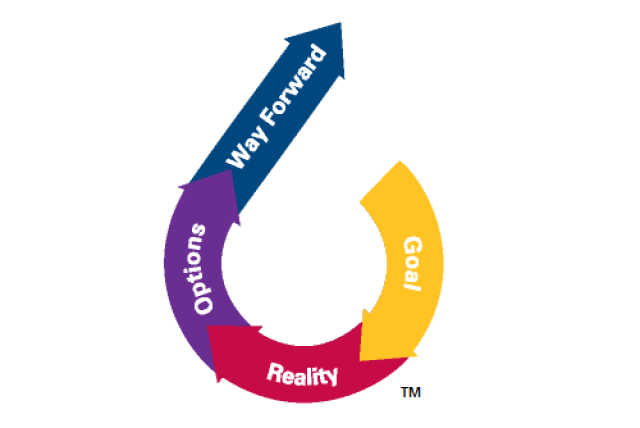
\includegraphics[width=0.7\textwidth]{GROW1}
		\label{fig:title}
	\end{figure}

\vspace{10mm}

		\begin{table}[!h]
		\centering
		\begin{tabular}{l c l}
			\textbf{Name:} & : & Timothy van der Steenhoven \\
				\textbf{Studentnumber} & : & $522397$ \\
				\textbf{E-mail} & : & 522397@student.inholland.nl \\
			\textbf{Course} & : & Honours Programm 1819\\
			\textbf{Study} &:& Applied Computer Science \\
			
		\end{tabular}	
	\end{table}

	\newpage
	
	\tableofcontents
	\vspace{10mm}
	\hrule
	
	\section*{Introduction}
	\paragraph{This} report is based on the first coaching session together with my coach Cees-Jeroen Bes. In this session we used the GROW Model made by Sir John Whitmore. 
	
	\paragraph{GROW} stands for Goal - Current Reality - Options - Will/Wrap-up. In the next chapter I will explain the goal I have discovered together with my coach. In chapter \ref{sec:CR} the current situation will be sketched. With a clear situation in mind, I can move on to chapter \ref{sec:Options}. Here I will present the possible options to get to my goal presented in chapter \ref{sec:Goals}. In the last chapter, chapter \ref{sec:Will} my Will to achieve my goal will be finalized. 
	
	\section{Goal}\label{sec:Goals}
	\paragraph{Together} with my coach I had a conversation about difficult situations within my study. These situations primarily exist in the projects I do for my study. I talked about having a difficult time with letting go of my responsibilities within the projects. 
	
	\paragraph{In} a project I almost always have a leading role. I like to make the plans at the beginning of the project and every week I do a little check-up with my fellow students on the project. This gives me a sense of safety and control. 
	
	\paragraph{The dark side} of having control is, in my case, that I cannot commit myself to a specific aspect of a project. This is because I have the idea:``If I do this myself, I know we can't get it wrong.'' , but in the past few months I have come to the conclusion that this is not an efficient thought. 
	
	\paragraph{Together} with my coach we have established that this keeps me from fulfilling my potential in a project. An important aspect later in life will be the know-how of trusting my colleagues in delivering a good job. 
	
	\paragraph{So} my goals becomes: 
	
	\textit{I want to fully trust my fellow students. I am aware that his means that I will be having less control, so I can fulfill my potential within our project.}
	
	\section{Current Reality}\label{sec:CR}
	\paragraph{With} the goal in mind, I can sketch the situation with my coach. Even if I do not want to admit it, Cees-Jeroen tells me that I am a control freak. We start a rather difficult conversation about trusting your fellow colleagues, because without trust, no one within a team can reach their full potential.
	
	\paragraph{The reason} I find it a difficult conversation, is that I like to have direct control of a situation. Sometimes it means that I will fully take over a problem, but actually it is a problem of the whole team. So I will have to face the fact that I can not always solve every problem.
	
	\paragraph{Another} important fact Cees-Jeroen tells me, is that I can influence a situation that I do not have direct control over. In the next chapter I will talk about that option. 
	
	\section{Explore the Options}\label{sec:Options}
	\paragraph{Indirect control.} Cees-Jeroen tells me that via an open dialog, people van influence each other in their work. Instead of saying ``We have to do it this way.'' I can ask ``What is the next step?''. The difference is that the last question opens a dialog and invites people to present their ideas.
	
	\paragraph{Working} towards an open dialog can give me some indirect control of a situation and can raise everybody their potential in a project. 
	
	\paragraph{A different} option for me, is to set up boundaries within a project. An example is making an agreement on how to communicate with one another, hopefully leading to an open dialog. 
	
	\paragraph{The last option} I have talked about with my coach, is developing my interpersonal skills. The main reason is, there are a lot of different people in the world and there are a lot of different approaches to a conversation. People also have alot of different potentials in different fields. 
	
	\paragraph{Knowing} which person is the best equipped for a job can greatly increase efficiency within a team and give me more confidence to trust in people.
	
	\paragraph{NOTE:} At the end of our coaching session I came to the conclusion that I like a immediate result after putting my trust in someone. Together with Cees-Jeroen I came to the conclusion that trust can be a long-term investment.  
	
	\section{Establish the Will}\label{sec:Will}
	\paragraph{This} is the last chapter of the GROW model. In this chapter I will think about the actions I have to take to get to my goal. 
	
	\paragraph{Firstly,} I will have to notice that the conversation I am having with a colleague is not an open dialog. A few example sentences: ``What do you think about this problem?'' and ``Can you please elaborate your decision?''. 
	
	\paragraph{Secondly,} evaluate with my teammates and ask them to hold up a mirror. A method that I can use is TIPS and TOPS.
	\begin{itemize}
		\item TIPS: Which advise can I take with me to the next project?
		\item TOPS: What did I do well?
	\end{itemize} 

	\paragraph{Lastly,} I should work on my interpersonal skills. This way I can be more prepared to establish an open dialog from the start and trust my colleagues/team mates/fellow students, in our projects.
	
	
	
	
	
	
	
	
	
	
	
	
	
\end{document}}